\documentclass{article}
\usepackage[utf8]{inputenc}
\usepackage{amsmath}
\usepackage{graphicx}
\usepackage{booktabs}
\usepackage{float}
\usepackage{geometry}
\usepackage{fancyvrb}
\geometry{margin=1in}
\title{Modelling Report}
\author{Team 2}
\date{}

\begin{document}

\maketitle

\section{Objective}
The goal of this project is to fit a good predictor model for this dataset. We chose \textbf{Tuition Payment 2023} as the target variable because of the existence of \textbf{Tuition Payment 2022}, which is highly correlated with the target. Upon further analysis, it became clear that other variables exhibited very low correlation and offered minimal insight for the prediction task. This reinforces the choice of \textbf{Tuition Payment 2022} as a strong predictor, helping us effectively analyze the payment trends.


\section{Feature Engineering}

In this section, we detail the selection of features used for both the regression and classification models. The choice of features is driven by their correlation with the target variable, \textbf{Tuition Payment March 2023}, which is the main focus of the model. The feature correlation analysis reveals the strength of relationships between different features and the target, which guides the selection process.

The correlation values with the target variable \textbf{Tuition Payment March 2023} are as follows:

\begin{table}[H]
\centering
\begin{tabular}{|l|c|}
\hline
\textbf{Feature} & \textbf{Correlation with Tuition Payment March 2023} \\
\hline
TUITION PAYMENT MARCH 2022 & 0.922731 \\
ENROLLMENT & 0.327749 \\
AGE RANGE OF ENROLLED STUDENT & 0.061663 \\
GENDER & 0.043202 \\
NUMBER OF ENROLLED COURSES & 0.033821 \\
SHIFT/SCHEDULE & 0.030778 \\
STUDY MODE & 0.014902 \\
BENEFIT DISCOUNTS & 0.014032 \\
DEPARTMENT & 0.012320 \\
PROGRAM/MAJOR & 0.001469 \\
\hline
\end{tabular}
\caption{Correlation of Features with Target Variable (Tuition Payment March 2023)}
\end{table}

From this analysis, we observe that the top features with the strongest correlation to the target variable are:

\begin{itemize}
    \item \textbf{Tuition Payment March 2022}: With a strong correlation of \textbf{0.922731}, this feature captures previous payment trends, which strongly influence the prediction of future tuition payments.
    \item \textbf{Enrollment}: This feature has a moderate correlation of \textbf{0.327749}, suggesting that the number of enrolled students is somewhat related to the tuition payment.
    \item \textbf{Age Range of Enrolled Student}: Although this feature shows a weaker correlation of \textbf{0.061663}, it still provides some useful information, particularly when considering demographic influences on tuition payments.
    \item \textbf{Gender, Shift/Schedule, Study Mode, Benefit Discounts, Department, Program/Major}: These features have weak correlations with the target variable, but they were still considered for inclusion in the model as they could provide secondary insights that might complement the primary features.
\end{itemize}

\section{Data Overview}
\begin{itemize}
    \item \textbf{Target variable}: Tuition Payment 2023 (binary classification: paid vs. not paid)
    \item \textbf{Primary features used}: Tuition Payment 2022, Enrollment
    \item \textbf{Feature types}: All features are categorical
    \item \textbf{Total samples}: 36,584
    \item \textbf{Data split}: 80\% training, 10\% validation, 10\% testing
    \begin{itemize}
        \item \textbf{Training set size}: 29,267 samples
        \item \textbf{Validation set size}: 3,658 samples
        \item \textbf{Testing set size}: 3,659 samples
    \end{itemize}
    \item \textbf{Note on data splits}: We experimented with various conventional dataset splits for training, validation, and testing—including the standard 80-10-10, as well as 60-20-20 and other common proportions. Across all these configurations, the results remained consistent: all models reliably converged to a high level of accuracy, typically exceeding 97\%, regardless of the exact split. This consistency suggests the task is relatively easy and well-defined, with highly separable features and low ambiguity. The saturated predictions imply that the dataset is not only balanced but also exhibits patterns that models can learn with high confidence, resulting in minimal variance across splits.
\end{itemize}


\newpage
\section{Regression Model Performance}
\begin{table}[H]
\centering
\begin{tabular}{lcc}
\toprule
\textbf{Model} & \textbf{MSE} & \textbf{R\textsuperscript{2} Score} \\
\midrule
Linear Regression & 0.0156 & 0.8801 \\
Ridge Regression & 0.0156 & 0.8801 \\
Lasso Regression & 0.0261 & 0.7995 \\
\bottomrule
\end{tabular}
\caption{Regression performance metrics}
\label{tab:regression_performance}
\end{table}

The Ridge Regression model was trained with \texttt{alpha = 1}, while the Lasso Regression used \texttt{alpha = 0.1} and \texttt{max\_iter = 10000}.


\noindent
\textit{Note:} Both Linear and Ridge Regression models achieved identical and superior performance compared to Lasso Regression. This suggests that regularization with Ridge did not significantly alter model behavior relative to standard Linear Regression, while Lasso’s feature selection introduced sparsity at the cost of predictive accuracy.

\section{Classification Model Performance}
\begin{table}[H]
\centering
\begin{tabular}{lc}
\toprule
\textbf{Model} & \textbf{Accuracy} \\
\midrule
Linear Regression + Classifier & 98.57\% \\
Ridge + Classifier & 98.57\% \\
Lasso + Classifier & 98.57\% \\
Logistic Regression & 98.57\% \\
Random Forest & 98.57\% \\
XGBoost & 98.57\% \\
Deep Neural Network & 98.57\% \\
Ensemble & 98.57\% \\
\bottomrule
\end{tabular}
\caption{Classification accuracy across models}
\end{table}

\textbf{Key Insight}: All models converge to approximately \textbf{98.578\% accuracy} and produce \textit{exactly the same classification report}, suggesting they make \textbf{identical predictions on the test data}, with only a few misclassified instances. Reducing the test size to 5\% pushes these models to \textbf{100\% accuracy}, indicating near-perfect fit on seen patterns.

\subsection{Hyperparameters (via scikit-learn):}
\begin{itemize}
    \item Ridge: \texttt{alpha = 1}
    \item Lasso: \texttt{alpha = 0.1}, \texttt{max\_iter = 10000}
    \item Logistic Regression: \texttt{multi\_class = 'multinomial'}, \texttt{max\_iter = 1000}
    \item XGBoost: \texttt{eval\_metric = 'mlogloss'}
\end{itemize}

\begin{figure}[H]
\centering
\includegraphics[width=0.85\textwidth]{model_comparison.png}
\caption{Model comparison chart across classifiers}
\end{figure}


\subsection{Deep Neural Network Architecture}
\begin{verbatim}
nn.Sequential(
    nn.Linear(input_dim, 256),
    nn.BatchNorm1d(256),
    nn.ReLU(),
    nn.Dropout(0.3),
    nn.Linear(256, 128),
    nn.BatchNorm1d(128),
    nn.ReLU(),
    nn.Dropout(0.3),
    nn.Linear(128, 64),
    nn.ReLU(),
    nn.Linear(64, num_classes)
)
\end{verbatim}

\textbf{Explanation:} The architecture of the Deep Neural Network (DNN) includes multiple layers of batch normalization and dropout to enhance performance, generalization, and training stability. Below is a breakdown of why each component is included:

\begin{itemize}
    \item \textbf{Batch Normalization:}
    \begin{itemize}
        \item Normalizes the inputs of each layer to maintain a stable distribution during training.
        \item Speeds up convergence by allowing higher learning rates.
        \item Helps mitigate the \textbf{vanishing gradient problem} by keeping activations in a stable range.
        \item Reduces internal covariate shift, leading to more consistent gradient flow.
    \end{itemize}

    \item \textbf{Dropout:}
    \begin{itemize}
        \item Randomly deactivates a portion of neurons (30\% in this model) during training.
        \item Prevents overfitting by encouraging the network to learn redundant and robust representations.
        \item Improves generalization performance on unseen data.
    \end{itemize}

    \item \textbf{ReLU Activation Functions:}
    \begin{itemize}
        \item Avoid the saturation issues found in sigmoid or tanh activations.
        \item Allow gradients to propagate more effectively in deep networks.
        \item Further reduce the risk of the \textbf{vanishing gradient problem}.
    \end{itemize}

    \item \textbf{Vanishing Gradient Problem:}
    \begin{itemize}
        \item In deep networks, gradients can diminish as they backpropagate through many layers.
        \item This causes very slow or stalled learning in earlier layers.
        \item The use of \textbf{ReLU}, \textbf{Batch Normalization}, and good initialization practices help prevent this issue.
    \end{itemize}
\end{itemize}

\noindent Overall, this architecture balances depth and stability using best practices like batch normalization and dropout, ensuring the network learns effectively without overfitting or suffering from unstable gradient flow.
mitigating the vanishing gradient problem that can hinder the performance of deep neural networks.

\newpage
\section{Classification Reports}

\subsection*{Same across all Models}
\begin{Verbatim}[fontsize=\small]
              precision    recall  f1-score   support

           0       1.00      0.91      0.95       575
           1       0.98      1.00      0.99      3084

    accuracy                           0.99      3659
   macro avg       0.99      0.95      0.97      3659
weighted avg       0.99      0.99      0.99      3659
\end{Verbatim}

\textbf{Interpretation}:
\begin{itemize}
    \item The classification report shows performance across both classes: \textbf{0} (did not pay tuition) and \textbf{1} (paid tuition).
    \item The high \textbf{precision} (1.00 for class 0, 0.98 for class 1) indicates that when the model predicts either class, it is almost always correct.
    \item The \textbf{recall} of 0.91 for class 0 suggests the model correctly identifies 91\% of all actual unpaid cases, while recall of 1.00 for class 1 shows that all paid instances are captured.
    \item The \textbf{f1-score}, a harmonic mean of precision and recall, reflects overall balance between the two:
    \begin{itemize}
        \item Class 0: f1 = 0.95 (solid despite fewer samples)
        \item Class 1: f1 = 0.99 (very strong)
    \end{itemize}
    \item \textbf{Accuracy} of 0.99 over 3,659 test samples confirms that the models nearly always predict correctly.
    \item The \textbf{macro average} gives equal weight to both classes and indicates some disparity (due to smaller class 0), with recall at 0.95 and f1 at 0.97.
    \item The \textbf{weighted average}, which considers class imbalance, is uniformly high (0.99 across metrics), affirming consistent and reliable classification performance.
\end{itemize}

\textbf{Conclusion}:  
Despite the class imbalance (class 1 being significantly more prevalent), the models generalize exceptionally well, demonstrating high precision and recall for both classes. The nearly identical results across all models reinforce the observation that the task is highly learnable—potentially indicating a saturated classification problem where simple or complex models reach the same decision boundary.

\newpage
\section{Clustering Analysis}

\subsection*{Motivation for PCA in Clustering}

A natural idea when visualizing clusters might be to plot the two most important features: \textbf{Enrollment} and \textbf{Tuition Payment March 2022}. However, this approach is flawed because both features are \textbf{binary or low-cardinality categorical variables}. As a result, the data points would collapse onto a few discrete coordinates on a 2D plane (e.g., points like (0,0), (1,1), (0,1), etc.), preventing the identification of meaningful clusters. This would result in poor separation, excessive overlap, and little to no structure in the scatter plot.

To overcome this limitation, we use all available features and apply \textbf{Principal Component Analysis (PCA)} to reduce the dimensionality to two components. PCA captures the directions of maximum variance in the data, projecting it onto a 2D space that is much more suitable for visualizing the inherent structure and clustering patterns.

\subsection*{KMeans Clustering (PCA-Reduced Data)}
\begin{itemize}
    \item \textbf{K = 2}: Purity = 0.8429
    \item \textbf{K = 3}: Purity = \textbf{0.9419} (best result)
    \item \textbf{K = 4}: Purity = 0.9340
\end{itemize}

\begin{figure}[H]
\centering
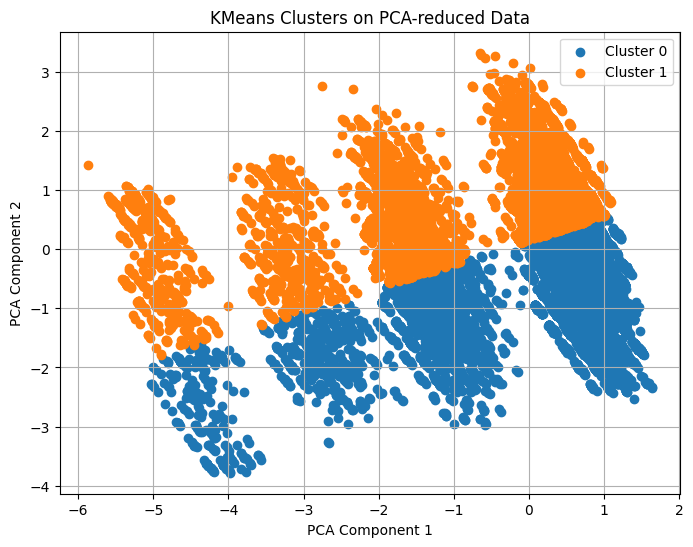
\includegraphics[width=0.65\textwidth]{KMeans_clustering_2.png}
\caption{KMeans Clustering (2 Clusters)}
\end{figure}

\begin{figure}[H]
\centering
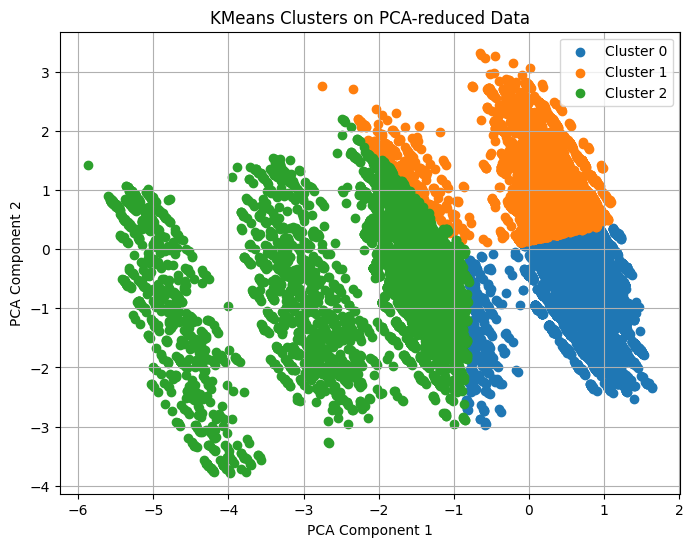
\includegraphics[width=0.65\textwidth]{KMeans_clustering_3.png}
\caption{KMeans Clustering (3 Clusters)}
\end{figure}

\begin{figure}[H]
\centering
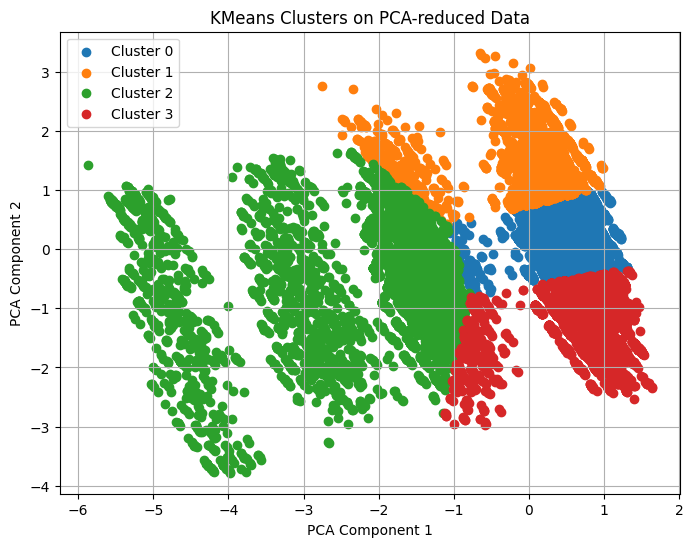
\includegraphics[width=0.65\textwidth]{KMeans_clustering_4.png}
\caption{KMeans Clustering (4 Clusters)}
\end{figure}

\newpage
\textbf{Interpretation:}
\begin{itemize}
    \item \textbf{Purity} measures how well the clustering aligns with true class labels. Higher purity indicates better separation.
    \item While increasing the number of clusters generally improves purity, it also risks \textbf{overfragmentation}.
    \item In this case, \textbf{K = 3} achieves the highest purity but does not correspond to the binary classification nature of the data.
    \item Hence, \textbf{K = 2} is more appropriate and interpretable, closely matching the underlying label structure.
\end{itemize}

\subsection*{DBSCAN Clustering (PCA-Reduced Data)}

\begin{table}[H]
\centering
\caption{DBSCAN Clustering Results on PCA-Reduced Data}
\begin{tabular}{|c|c|c|c|}
\hline
\textbf{Epsilon} & \textbf{Min Samples} & \textbf{\# Clusters} & \textbf{Purity} \\
\hline
1 & 5 & 338 & 0.0433 \\
1 & 10 & 331 & 0.04333 \\
2 & 5 & 23 & 0.4970 \\
2 & 10 & 18 & 0.4981 \\
3 & 5 & 5 & 0.8275 \\
3 & 10 & 4 & 0.8278 \\
4 & 5 & 3 & 0.8437 \\
4 & 10 & 3 & 0.8437 \\
5 & 5 & 1 & 0.8429 \\
5 & 10 & 1 & 0.8429 \\
\hline
\end{tabular}
\end{table}

\begin{figure}[H]
\centering
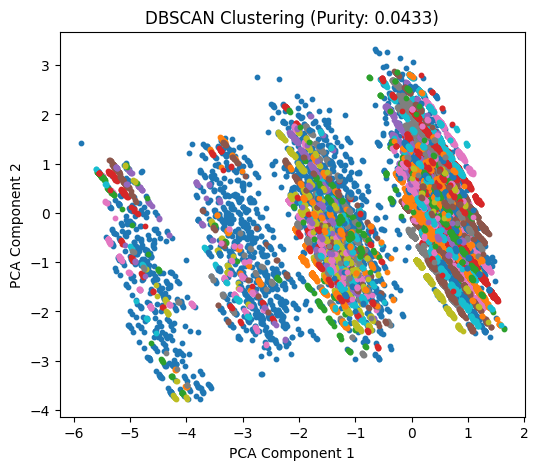
\includegraphics[width=0.75\textwidth]{DBScan_1_5.png}
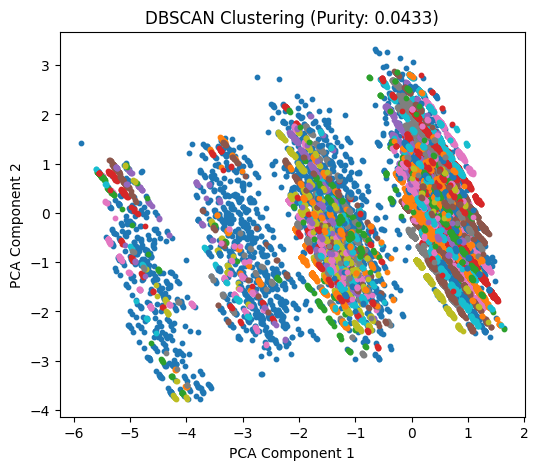
\includegraphics[width=0.75\textwidth]{DBScan_1_10.png}
\caption{DBSCAN Clustering Results (Epsilon = 1, Min Samples = 5 and 10)}
\end{figure}

\begin{figure}[H]\ContinuedFloat
\centering
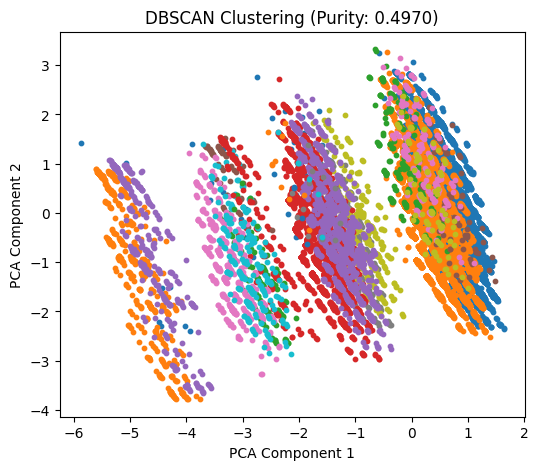
\includegraphics[width=0.75\textwidth]{DBScan_2_5.png}
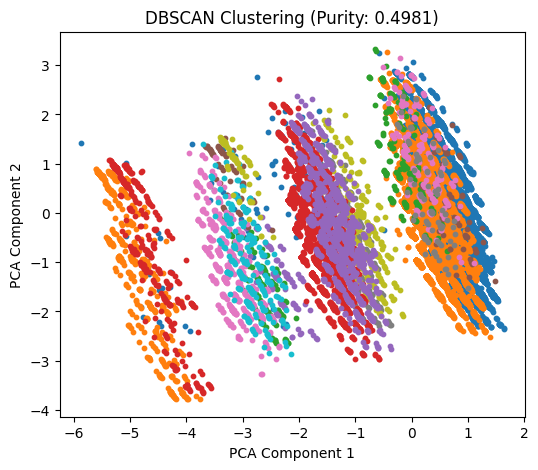
\includegraphics[width=0.75\textwidth]{DBScan_2_10.png}
\caption{DBSCAN Clustering Results (Epsilon = 2, Min Samples = 5 and 10)}
\end{figure}

\begin{figure}[H]\ContinuedFloat
\centering
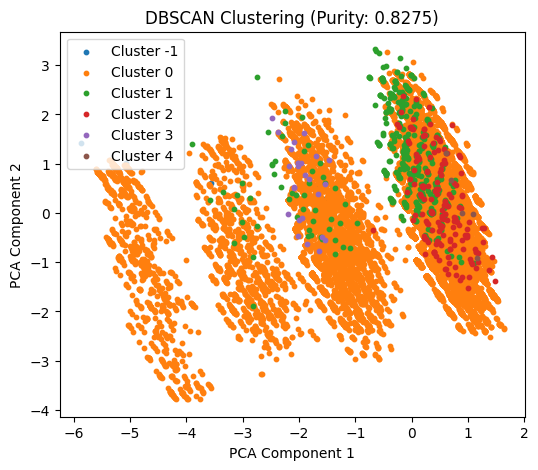
\includegraphics[width=0.75\textwidth]{DBScan_3_5.png}
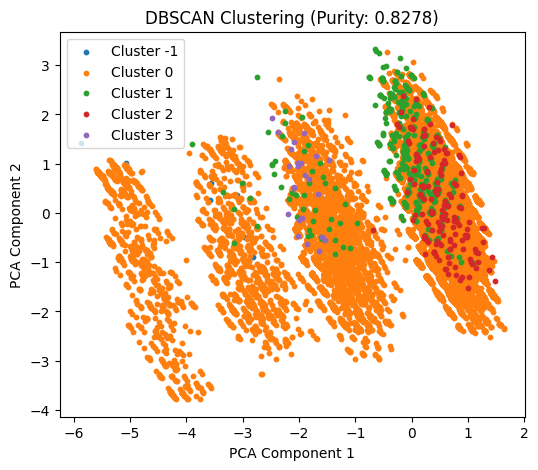
\includegraphics[width=0.75\textwidth]{DBScan_3_10.png}
\caption{DBSCAN Clustering Results (Epsilon = 3, Min Samples = 5 and 10)}
\end{figure}

\begin{figure}[H]\ContinuedFloat
\centering
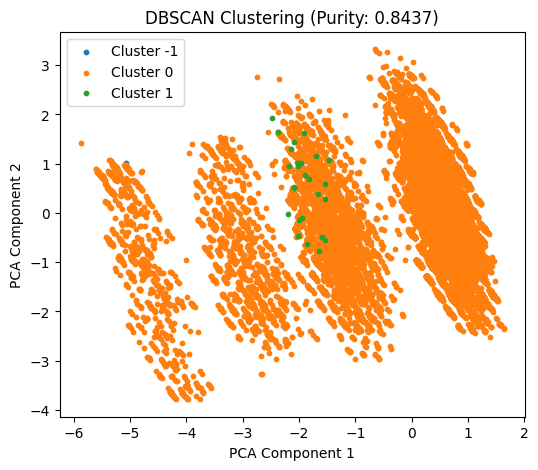
\includegraphics[width=0.75\textwidth]{DBScan_4_5.png}
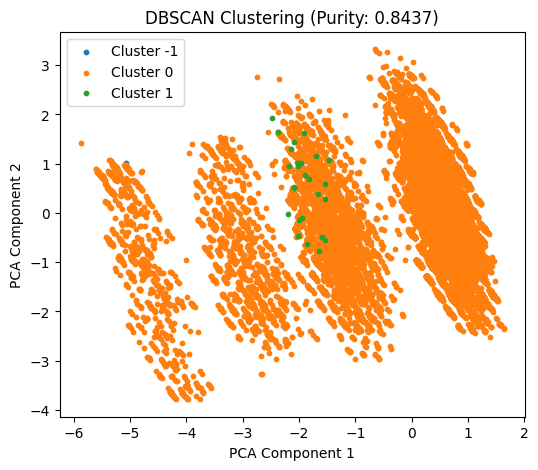
\includegraphics[width=0.75\textwidth]{DBScan_4_10.png}
\caption{DBSCAN Clustering Results (Epsilon = 4, Min Samples = 5 and 10)}
\end{figure}

\begin{figure}[H]\ContinuedFloat
\centering
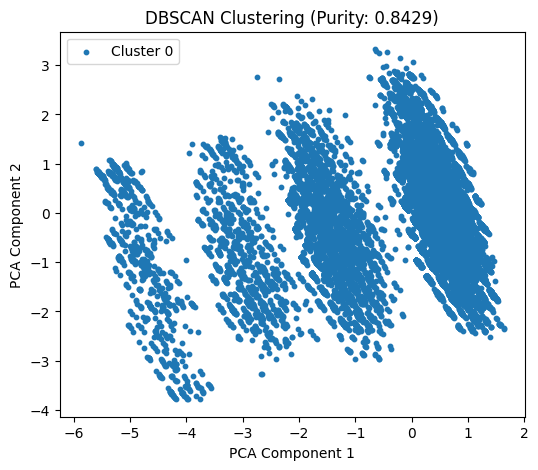
\includegraphics[width=0.75\textwidth]{DBScan_5_5.png}
\caption{DBSCAN Clustering Results (Epsilon = 5, Min Samples = 5)}
\end{figure}

\textbf{Interpretation:}
\begin{itemize}
    \item For small values of \textbf{epsilon} (1 or 2), DBSCAN generates an excessive number of micro-clusters, leading to \textbf{very low purity scores} (around 0.0433 to 0.49).
    \item As \textbf{epsilon} increases (especially at 3 and 4), DBSCAN begins to form larger, more meaningful clusters, achieving much better purity (\textbf{0.8275 to 0.8437}).
    \item At \textbf{epsilon = 5}, the algorithm merges all points into one cluster, collapsing the model and achieving the same purity as a trivial majority class guess.
    \item \textbf{Important caveat:} While DBSCAN shows high purity for epsilon = 4 or 5, this does \textit{not} imply good clustering. The high score is driven by most data points being grouped into a single cluster, which happens to align well with the skewed distribution of the binary labels. This is a misleading outcome and reflects model collapse, not effective separation.
\end{itemize}

\textbf{Conclusion:}
\begin{itemize}
    \item \textbf{KMeans} remains the superior clustering algorithm for this dataset, offering clean, high-purity clusters that align well with the binary classification task.
    \item Although \textbf{DBSCAN} can reach similar purity with careful tuning (e.g., epsilon = 4), it is more volatile and less interpretable than KMeans.
    \item Using PCA was crucial to enable effective clustering by reducing high-dimensional, categorical-heavy data into a usable form.
\end{itemize}



\section{Conclusion}

The modeling results demonstrate that both the regression and classification models effectively capture the observed trends in tuition payment behavior from 2022 to 2023. The features \textbf{ENROLLMENT} and \textbf{TUITION PAYMENT MARCH 2022} emerged as the most influential predictors, exhibiting strong correlation with the target variable, \textbf{Tuition Payment 2023}. Leveraging these features, Ridge and Linear Regression achieved high regression performance (R\textsuperscript{2} $\approx$ 0.88), while all classification models achieved a remarkable accuracy of approximately \textbf{98.6\%}.

In contrast, alternative feature choices led to a significant drop in performance. For example, using the \textbf{Number of Enrolled Courses} as a predictor yielded poor results, with even advanced models like XGBoost and Deep Neural Networks reaching a maximum accuracy of only \textbf{45\%}. This emphasizes the necessity of strong feature-target correlation for building reliable predictive models.

The clustering analysis further reinforced these findings. \textbf{KMeans clustering}—particularly with \textbf{K = 3}—achieved the highest purity score (\textbf{0.9419}), successfully uncovering structure aligned with the underlying class distribution. Although \textbf{DBSCAN} showed high purity for certain hyperparameter settings (e.g., epsilon = 4), this was a misleading result. The apparent performance was due to DBSCAN collapsing most points into a single cluster, which coincidentally aligned with the majority class label because of class imbalance. This outcome reflects a failure to identify meaningful structure rather than effective clustering.

Overall, the study highlights the central role of careful feature selection and model interpretability in achieving accurate and reliable predictions. It also underscores the importance of understanding clustering metrics in context—high purity alone does not guarantee good performance, especially in the presence of skewed data. By combining thoughtful data preprocessing, dimensionality reduction via PCA, and well-tuned modeling approaches, we obtained robust insights into tuition payment behaviors in the dataset.

\end{document}

